\documentclass{standalone}
\usepackage{pgf,tikz}

\begin{document}

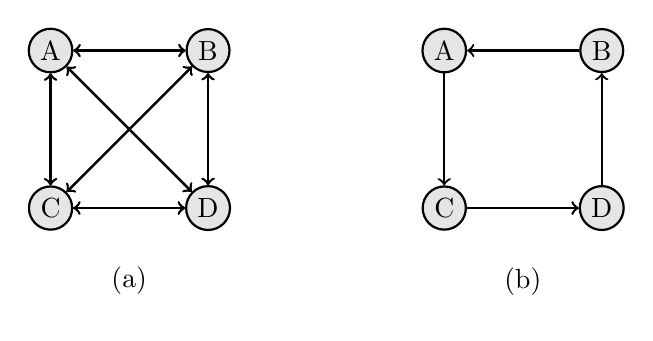
\begin{tikzpicture}
  [scale=0.5,every node/.style={circle, thick, draw=black,fill=black!10,inner sep=2pt}]
  
  %%%%%%%%%%%%%%%%%%%%%% ROW 1 %%%%%%%%%%%%%%%%%%%%%% 
  
  \node (comp_1) at (0,4)  		{A};
  \node(comp_2) at (4,4)  		{B};
  \node(comp_3) at (0,0)  		{C};
  \node (comp_4) at (4,0)  		{D};
  
  \node (circ_1) at (10,4)  		{A};
  \node(circ_2) at (14,4)  			{B};
  \node(circ_3) at (10,0)  			{C};
  \node (circ_4) at (14,0)  		{D};
 
  \foreach \fromcomp/\tocomp in {comp_1/comp_2,comp_1/comp_3,comp_1/comp_4,comp_2/comp_1,comp_2/comp_3,comp_2/comp_4,comp_3/comp_1,comp_3/comp_2,comp_3/comp_4,comp_4/comp_1,comp_4/comp_2,comp_4/comp_3}
    \draw[<->, thick] (\fromcomp) -- (\tocomp);
    
     \foreach \fromcirc/\tocirc in {circ_2/circ_1,circ_1/circ_3,circ_3/circ_4,circ_4/circ_2}
    \draw[->, thick] (\fromcirc) -- (\tocirc);
    
        \draw[->, thick]  (comp_3) -- (comp_4) node [draw=none,fill=none,midway,below=15pt] {(a)};
	        \draw[->, thick]  (circ_3) -- (circ_4) node [draw=none,fill=none,midway,below=15pt] {(b)};

          	
\end{tikzpicture}
\end{document}